% Created by tikzDevice version 0.12.6 on 2024-08-15 14:44:41
% !TEX encoding = UTF-8 Unicode
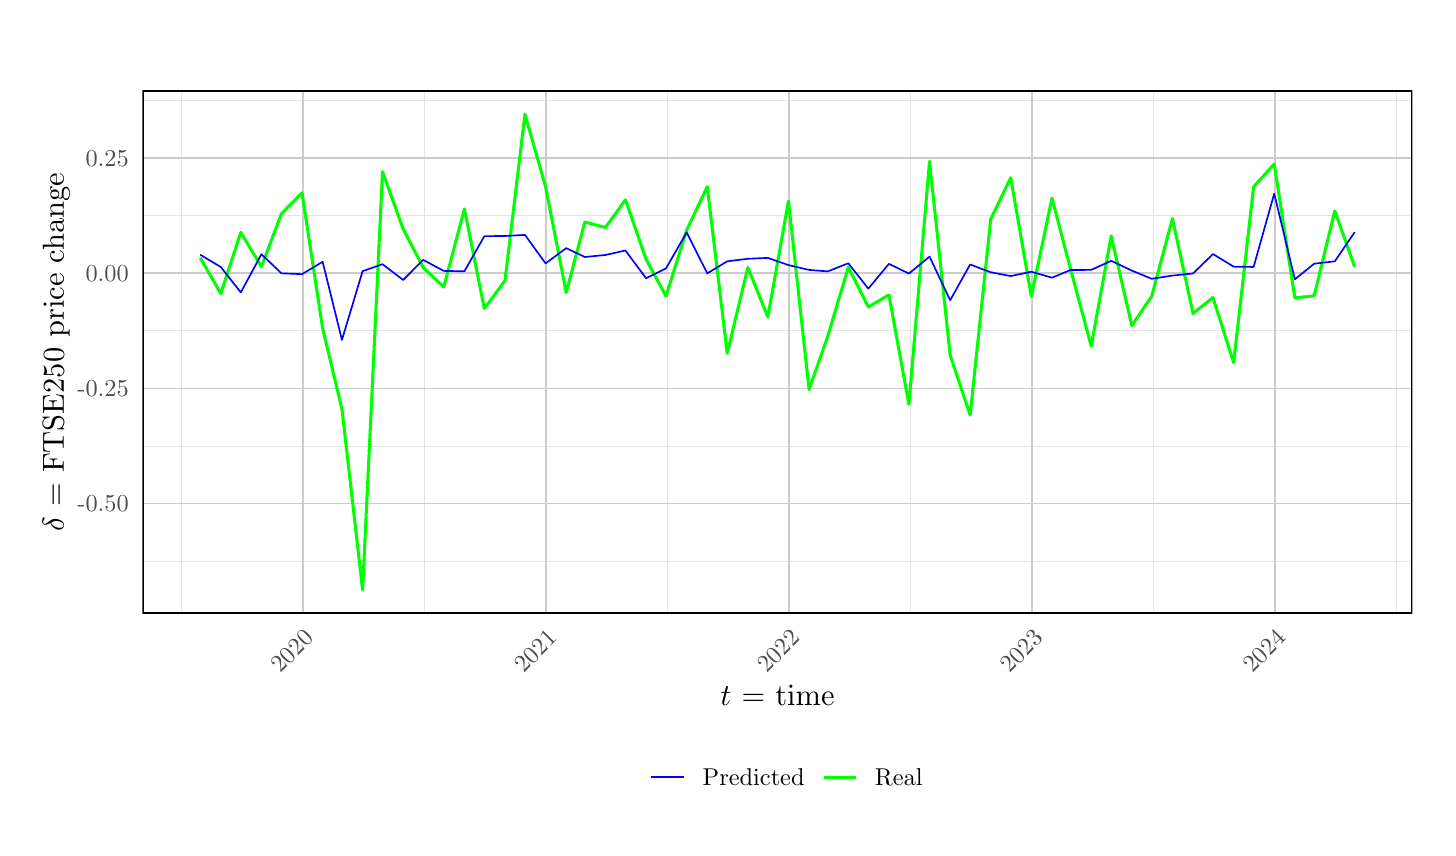
\begin{tikzpicture}[x=1pt,y=1pt]
\definecolor{fillColor}{RGB}{255,255,255}
\path[use as bounding box,fill=fillColor,fill opacity=0.00] (0,0) rectangle (505.89,289.08);
\begin{scope}
\path[clip] ( 41.49, 77.31) rectangle (500.39,266.42);
\definecolor{drawColor}{gray}{0.90}

\path[draw=drawColor,line width= 0.3pt,line join=round] ( 41.49, 96.28) --
	(500.39, 96.28);

\path[draw=drawColor,line width= 0.3pt,line join=round] ( 41.49,137.92) --
	(500.39,137.92);

\path[draw=drawColor,line width= 0.3pt,line join=round] ( 41.49,179.57) --
	(500.39,179.57);

\path[draw=drawColor,line width= 0.3pt,line join=round] ( 41.49,221.21) --
	(500.39,221.21);

\path[draw=drawColor,line width= 0.3pt,line join=round] ( 41.49,262.86) --
	(500.39,262.86);

\path[draw=drawColor,line width= 0.3pt,line join=round] ( 55.49, 77.31) --
	( 55.49,266.42);

\path[draw=drawColor,line width= 0.3pt,line join=round] (143.38, 77.31) --
	(143.38,266.42);

\path[draw=drawColor,line width= 0.3pt,line join=round] (231.26, 77.31) --
	(231.26,266.42);

\path[draw=drawColor,line width= 0.3pt,line join=round] (319.03, 77.31) --
	(319.03,266.42);

\path[draw=drawColor,line width= 0.3pt,line join=round] (406.79, 77.31) --
	(406.79,266.42);

\path[draw=drawColor,line width= 0.3pt,line join=round] (494.68, 77.31) --
	(494.68,266.42);
\definecolor{drawColor}{gray}{0.80}

\path[draw=drawColor,line width= 0.6pt,line join=round] ( 41.49,117.10) --
	(500.39,117.10);

\path[draw=drawColor,line width= 0.6pt,line join=round] ( 41.49,158.75) --
	(500.39,158.75);

\path[draw=drawColor,line width= 0.6pt,line join=round] ( 41.49,200.39) --
	(500.39,200.39);

\path[draw=drawColor,line width= 0.6pt,line join=round] ( 41.49,242.04) --
	(500.39,242.04);

\path[draw=drawColor,line width= 0.6pt,line join=round] ( 99.38, 77.31) --
	( 99.38,266.42);

\path[draw=drawColor,line width= 0.6pt,line join=round] (187.38, 77.31) --
	(187.38,266.42);

\path[draw=drawColor,line width= 0.6pt,line join=round] (275.15, 77.31) --
	(275.15,266.42);

\path[draw=drawColor,line width= 0.6pt,line join=round] (362.91, 77.31) --
	(362.91,266.42);

\path[draw=drawColor,line width= 0.6pt,line join=round] (450.68, 77.31) --
	(450.68,266.42);
\definecolor{drawColor}{RGB}{0,255,0}

\path[draw=drawColor,line width= 1.1pt,line join=round] ( 62.35,205.92) --
	( 69.80,193.01) --
	( 77.01,215.09) --
	( 84.47,202.69) --
	( 91.68,221.81) --
	( 99.14,229.38) --
	(106.59,180.36) --
	(113.56,151.33) --
	(121.02, 85.90) --
	(128.23,237.03) --
	(135.68,216.32) --
	(142.90,202.45) --
	(150.35,195.34) --
	(157.81,223.55) --
	(165.02,187.59) --
	(172.47,197.66) --
	(179.69,257.83) --
	(187.14,231.57) --
	(194.60,193.36) --
	(201.33,218.85) --
	(208.78,216.86) --
	(216.00,226.88) --
	(223.45,205.44) --
	(230.66,192.06) --
	(238.12,215.90) --
	(245.57,231.61) --
	(252.78,171.41) --
	(260.24,202.43) --
	(267.45,184.51) --
	(274.91,226.41) --
	(282.36,158.32) --
	(289.09,177.51) --
	(296.55,202.53) --
	(303.76,188.17) --
	(311.21,192.52) --
	(318.43,152.99) --
	(325.88,240.78) --
	(333.34,170.75) --
	(340.55,149.09) --
	(348.00,219.92) --
	(355.22,234.86) --
	(362.67,191.99) --
	(370.13,227.47) --
	(376.86,201.74) --
	(384.31,174.00) --
	(391.53,213.84) --
	(398.98,181.39) --
	(406.19,192.11) --
	(413.65,220.07) --
	(421.10,185.83) --
	(428.31,191.56) --
	(435.77,168.01) --
	(442.98,231.53) --
	(450.44,239.81) --
	(457.89,191.42) --
	(464.86,192.19) --
	(472.32,222.85) --
	(479.53,202.58);
\definecolor{drawColor}{RGB}{0,0,255}

\path[draw=drawColor,line width= 0.6pt,line join=round] ( 62.35,207.04) --
	( 69.80,202.58) --
	( 77.01,193.41) --
	( 84.47,207.21) --
	( 91.68,200.32) --
	( 99.14,200.01) --
	(106.59,204.48) --
	(113.56,176.23) --
	(121.02,201.09) --
	(128.23,203.61) --
	(135.68,197.91) --
	(142.90,205.17) --
	(150.35,201.19) --
	(157.81,201.04) --
	(165.02,213.74) --
	(172.47,213.80) --
	(179.69,214.20) --
	(187.14,203.90) --
	(194.60,209.41) --
	(201.33,206.21) --
	(208.78,206.94) --
	(216.00,208.57) --
	(223.45,198.53) --
	(230.66,202.09) --
	(238.12,215.10) --
	(245.57,200.30) --
	(252.78,204.65) --
	(260.24,205.57) --
	(267.45,205.89) --
	(274.91,203.29) --
	(282.36,201.54) --
	(289.09,201.01) --
	(296.55,203.94) --
	(303.76,194.77) --
	(311.21,203.74) --
	(318.43,200.22) --
	(325.88,206.35) --
	(333.34,190.58) --
	(340.55,203.50) --
	(348.00,200.70) --
	(355.22,199.32) --
	(362.67,200.88) --
	(370.13,198.74) --
	(376.86,201.52) --
	(384.31,201.55) --
	(391.53,204.83) --
	(398.98,201.30) --
	(406.19,198.34) --
	(413.65,199.50) --
	(421.10,200.25) --
	(428.31,207.28) --
	(435.77,202.72) --
	(442.98,202.61) --
	(450.44,229.12) --
	(457.89,198.15) --
	(464.86,203.79) --
	(472.32,204.65) --
	(479.53,215.21);
\definecolor{drawColor}{RGB}{0,0,0}

\path[draw=drawColor,line width= 1.1pt,line join=round,line cap=round] ( 41.49, 77.31) rectangle (500.39,266.42);
\end{scope}
\begin{scope}
\path[clip] (  0.00,  0.00) rectangle (505.89,289.08);
\definecolor{drawColor}{gray}{0.30}

\node[text=drawColor,anchor=base east,inner sep=0pt, outer sep=0pt, scale=  0.88] at ( 36.54,114.07) {-0.50};

\node[text=drawColor,anchor=base east,inner sep=0pt, outer sep=0pt, scale=  0.88] at ( 36.54,155.72) {-0.25};

\node[text=drawColor,anchor=base east,inner sep=0pt, outer sep=0pt, scale=  0.88] at ( 36.54,197.36) {0.00};

\node[text=drawColor,anchor=base east,inner sep=0pt, outer sep=0pt, scale=  0.88] at ( 36.54,239.01) {0.25};
\end{scope}
\begin{scope}
\path[clip] (  0.00,  0.00) rectangle (505.89,289.08);
\definecolor{drawColor}{gray}{0.30}

\node[text=drawColor,rotate= 45.00,anchor=base east,inner sep=0pt, outer sep=0pt, scale=  0.88] at (103.66, 68.07) {2020};

\node[text=drawColor,rotate= 45.00,anchor=base east,inner sep=0pt, outer sep=0pt, scale=  0.88] at (191.67, 68.07) {2021};

\node[text=drawColor,rotate= 45.00,anchor=base east,inner sep=0pt, outer sep=0pt, scale=  0.88] at (279.43, 68.07) {2022};

\node[text=drawColor,rotate= 45.00,anchor=base east,inner sep=0pt, outer sep=0pt, scale=  0.88] at (367.20, 68.07) {2023};

\node[text=drawColor,rotate= 45.00,anchor=base east,inner sep=0pt, outer sep=0pt, scale=  0.88] at (454.96, 68.07) {2024};
\end{scope}
\begin{scope}
\path[clip] (  0.00,  0.00) rectangle (505.89,289.08);
\definecolor{drawColor}{RGB}{0,0,0}

\node[text=drawColor,anchor=base,inner sep=0pt, outer sep=0pt, scale=  1.10] at (270.94, 44.09) {$t$ = time};
\end{scope}
\begin{scope}
\path[clip] (  0.00,  0.00) rectangle (505.89,289.08);
\definecolor{drawColor}{RGB}{0,0,0}

\node[text=drawColor,rotate= 90.00,anchor=base,inner sep=0pt, outer sep=0pt, scale=  1.10] at ( 13.08,171.86) {$\delta$ = FTSE250 price change};
\end{scope}
\begin{scope}
\path[clip] (  0.00,  0.00) rectangle (505.89,289.08);
\definecolor{drawColor}{RGB}{0,0,255}

\path[draw=drawColor,line width= 0.6pt,line join=round] (225.41, 18.23) -- (236.98, 18.23);
\end{scope}
\begin{scope}
\path[clip] (  0.00,  0.00) rectangle (505.89,289.08);
\definecolor{drawColor}{RGB}{0,255,0}

\path[draw=drawColor,line width= 1.1pt,line join=round] (287.67, 18.23) -- (299.24, 18.23);
\end{scope}
\begin{scope}
\path[clip] (  0.00,  0.00) rectangle (505.89,289.08);
\definecolor{drawColor}{RGB}{0,0,0}

\node[text=drawColor,anchor=base west,inner sep=0pt, outer sep=0pt, scale=  0.88] at (243.92, 15.20) {Predicted};
\end{scope}
\begin{scope}
\path[clip] (  0.00,  0.00) rectangle (505.89,289.08);
\definecolor{drawColor}{RGB}{0,0,0}

\node[text=drawColor,anchor=base west,inner sep=0pt, outer sep=0pt, scale=  0.88] at (306.18, 15.20) {Real};
\end{scope}
\end{tikzpicture}
